\section{动力学}

\subsection{连接体问题}

\subsubsection{动滑轮}

\begin{proset}
    （多选）
    如图所示，离地足够高的轻质动滑轮下方悬挂质量为\(3m\)的重物\(P\)，轻质定滑轮下方悬挂质量为\(m\)的重物\(Q\)，悬挂滑轮的轻质细线竖直。开始时，\(P\)、\(Q\)均处于静止状态，不计摩擦阻力和空气阻力，重力加速度大小为\(g\)。释放后\paren[]

    \begin{tikzpicture}[font=\scriptsize]
        \draw[fill=gray!40] (0,0) circle(.3) (.6,1.5) circle(.3);
        \draw (0,0) circle(.25) (0,0) circle(.1) (.6,1.5) circle(.25) (.6,1.5) circle(.1);
        \draw[purple] (-.3,2)--(-.3,0) (.3,0)--(.3,1.5) (.9,1.5)--(.9,-1)coordinate(q) (0,0)--(0,-1)coordinate(p);
        \fill (0,0) circle(.05) (.6,1.5) circle(.05);
        \draw[fill=orange!40] ($(p)+(-.15,0)$) rectangle ($(p)+(.15,-.3)$)node[midway]{\(P\)} ($(q)+(-.15,0)$) rectangle ($(q)+(.15,-.3)$)node[midway]{\(Q\)};
        \foreach \x in{-.8,-.6,...,1.2}
            \draw[gray] (\x,2.2)--++(.2,-.2);
        \draw[thick] (-.8,2)--(1.4,2) (.6,1.5)--(.6,2);
    \end{tikzpicture}
    \begin{choices}
        \item \(Q\)受到细线拉力大小为\(mg\)
        \item \(Q\)受到细线拉力大小为\(\frac{9mg}{7}\)
        \item 当\(P\)位移大小为\(h\)时，\(Q\)的速度大小为\(\frac{\sqrt{2gh}}{2} \) 
        \item 当\(P\)位移大小为\(h\)时，\(Q\)的速度大小为\(\frac{2\sqrt{14gh}}{7} \)
    \end{choices}
\end{proset}
\begin{answer}
    BD\quad 提示：\(Q\)上升高度是\(P\)下降高度的2倍，\(Q\)的加速度和速度均是 \(P\)的2倍

    \(3mg - 2T = 3m\cdot a\)\quad \(T - mg = m\cdot 2a\)联立可得：\(T = \frac{9mg}{7}\)

    \(3mg\cdot h - mg\cdot 2h = \frac{1}{2} 3mv^2 + \frac{1}{2} m (2v)^2\)可得：\(v = \frac{\sqrt{14gh}}{7} \)
\end{answer}

\begin{proset}
    （多选）
    如图所示，质量为\(3m\)的物块\(A\)放在光滑的水平面上，轻绳的一端固定在物块\(A\)，另一端绕过两个光滑滑轮与质量为\(m\)的物块\(B\)相连，物块\(B\)与物块\(A\)紧挨在一起，两者接触面光滑，物块\(B\)一边下落一边随着物块\(A\)向右运动。重力加速度大小为\(g\)，滑轮质量不计，在物块\(B\)与地面接触之前，下列说法正确的是\paren[]

    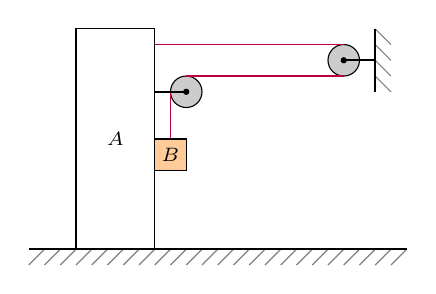
\begin{tikzpicture}[font=\scriptsize]
        \draw[fill=gray!40] (0,0) circle(.2) (2,.4) circle(.2);
        \draw[purple] (-.4,.6)--(2,.6) (2,.2)--(0,.2) (-.2,0)--(-.2,-.6);
        \draw[fill=orange!40] (-.4,-.6) rectangle(0,-1)node[midway]{\(B\)};
        \draw (-.4,.8) rectangle(-1.4,-2)node[midway]{\(A\)};
        \fill (0,0) circle(.04) (2,.4) circle(.04);
        \foreach \x in{-2,-1.8,...,2.6}
            \draw[gray] (\x,-2.2)--++(.2,.2);
        \foreach \y in{0,.2,...,.6}
            \draw[gray] (2.6,\y)--++(-.2,.2);
        \draw[thick] (2,.4)--(2.4,.4) (-.4,0)--(0,0) (-2,-2)--(2.8,-2) (2.4,0)--(2.4,.8);
    \end{tikzpicture}
    \begin{choices}
        \item 物块\(A\)、\(B\)的加速度大小相等
        \item 物块\(B\)的加速度大小等于\(\frac{\sqrt{5}}{4}g \)
        \item 物块\(A\)、\(B\)间的弹力大小等于\(\frac{1}{4}mg\)
        \item 绳子上的拉力大小等于\(\frac{\sqrt{5}}{2}g \)
    \end{choices}
\end{proset}
\begin{answer}
    BC\quad 提示：
\end{answer}